\documentclass[a4paper,11pt]{article}
\usepackage[T1]{fontenc}
\usepackage[utf8]{inputenc}
\usepackage{lmodern}
\usepackage[francais]{babel}

% title info
\newcommand{\ititle}{Rapport NF11} % title
\newcommand{\isubtitle}{Projet LOGO}
\newcommand{\iauthor}{\textsc{Impellettieri} Florian\\\textsc{Hammi} Marouane}% author
\newcommand{\idate}{\today} % date

\usepackage{graphicx}
\usepackage{tabularx}
\usepackage{lastpage}
\usepackage[top=2.75cm, bottom=3cm, left=2cm, right=2cm]{geometry}
\usepackage[colorlinks=true, urlcolor=blue, linkcolor=black, citecolor=black]{hyperref}
\usepackage{calc}
\usepackage{amsmath} % equation align
\usepackage{amsfonts}
\usepackage{amssymb}
% \usepackage{mathastext} % use \text{} when needed instead
\usepackage{fancyhdr}
\usepackage[format=hang, width=.8\textwidth, labelfont=sc]{caption}
\usepackage[format=hang, width=.8\textwidth, labelfont=normalfont]{subcaption}
% \usepackage[labelformat=empty]{caption} % no label before caption
\usepackage{verbatim}
\usepackage{framed}

% paragraph and subparagraph as level 4 and 5 sections
\usepackage{titlesec}
\usepackage{titletoc}
\setcounter{secnumdepth}{5}
\setcounter{tocdepth}{5}
\titleformat{\paragraph} [hang] {\normalfont\normalsize\bfseries} {\theparagraph} {1em} {}
\titleformat{\subparagraph} [hang] {\normalfont\normalsize\bfseries} {\thesubparagraph} {1em} {}

% lists config
\usepackage{enumitem}
\setlist[itemize]{label=-}

% replace no-break space
\DeclareUnicodeCharacter{00A0}{ }

% header & footer
\pagestyle{fancy}
\fancyhf{}
\setlength{\headheight}{14pt}
\lhead{{\small \ititle}}
\rhead{{\small Projet Logo}}
\lfoot{}
\rfoot{\hrule\vspace{.1cm}\thepage /\pageref*{LastPage}}

\usepackage{color}
\usepackage{xcolor}
\usepackage{listings}

% define colors
\definecolor{kblue}{HTML}{204A87}
\definecolor{cred}{HTML}{A52A2A}
\definecolor{sorange}{HTML}{FF7800}
\definecolor{ngreen}{HTML}{4E9A06}
\definecolor{pprocess}{HTML}{339999}
\definecolor{opbrown}{HTML}{AB7A00}

% code highlight style
\lstdefinestyle{lstyle}{
	aboveskip=9mm,
	belowskip=1mm,
	basicstyle=\ttfamily\footnotesize,
	keywordstyle=\bfseries\color{kblue},
	commentstyle=\color{cred},
	stringstyle=\color{sorange},
	emphstyle=\color{pprocess},
	breaklines=true,
	tabsize=3,
	showstringspaces=false,
	captionpos=b
% 	literate={=}{{{\color{opbrown}=}}}1
}

% language
\lstset{
	language=Java,
	frame=single,
	numbers=left,
	numberstyle=\footnotesize,
	style=lstyle,
	emph={},
	morekeywords={None, False, True},
	extendedchars=true
}

% utf8 char
\lstset{literate=
  {á}{{\'a}}1 {é}{{\'e}}1 {í}{{\'i}}1 {ó}{{\'o}}1 {ú}{{\'u}}1
  {Á}{{\'A}}1 {É}{{\'E}}1 {Í}{{\'I}}1 {Ó}{{\'O}}1 {Ú}{{\'U}}1
  {à}{{\`a}}1 {è}{{\`e}}1 {ì}{{\`i}}1 {ò}{{\`o}}1 {ù}{{\`u}}1
  {À}{{\`A}}1 {È}{{\'E}}1 {Ì}{{\`I}}1 {Ò}{{\`O}}1 {Ù}{{\`U}}1
  {ä}{{\"a}}1 {ë}{{\"e}}1 {ï}{{\"i}}1 {ö}{{\"o}}1 {ü}{{\"u}}1
  {Ä}{{\"A}}1 {Ë}{{\"E}}1 {Ï}{{\"I}}1 {Ö}{{\"O}}1 {Ü}{{\"U}}1
  {â}{{\^a}}1 {ê}{{\^e}}1 {î}{{\^i}}1 {ô}{{\^o}}1 {û}{{\^u}}1
  {Â}{{\^A}}1 {Ê}{{\^E}}1 {Î}{{\^I}}1 {Ô}{{\^O}}1 {Û}{{\^U}}1
  {œ}{{\oe}}1 {Œ}{{\OE}}1 {æ}{{\ae}}1 {Æ}{{\AE}}1 {ß}{{\ss}}1
  {ç}{{\c c}}1 {Ç}{{\c C}}1 {ø}{{\o}}1 {å}{{\r a}}1 {Å}{{\r A}}1
  {€}{{\EUR}}1 {£}{{\pounds}}1
}

% use with \begin{lstlisting}[caption={#}, language=#] # \end{lstlisting}
% or \lstinline[caption={#}, language=#]$#$ --> $ can be replaced by any other character not used in the code


\begin{document}
% title
\begin{center}
	\vspace*{.75cm}{\huge \textsc{\ititle}}~\\
	\vspace{.25cm}{\LARGE \isubtitle}~\\
	\vspace{.6cm}{\large\iauthor}~\\
	\vspace{.6cm}{\large\idate}
\end{center}
\vspace*{-1.5cm}

% logo
\vspace{\fill}
\hspace{-1.25cm}
\includegraphics[width=5cm]{img/utc-logo.jpg}
\vspace*{-1.5cm}

\thispagestyle{empty}

% table of content (newpage)
\newpage
\tableofcontents

% blue links after table of contents
\hypersetup{linkcolor=blue}

% section config
\titlespacing{\section}{0mm}{6mm}{0mm}
\titlespacing{\subsection}{0mm}{6mm}{0mm}
\titlespacing{\subsubsection}{0mm}{6mm}{0mm}
\titlespacing{\paragraph}{0mm}{6mm}{0mm}
\titlespacing{\subparagraph}{0mm}{6mm}{0mm}

% paragraph config
\setlength{\parindent}{0mm}
\setlength{\parskip}{6mm}


\newpage
\section{Introduction}

\subsection{Contexte}
Ce document constitue le rapport du projet de NF11. Au cours de ce projet l'objectif a été de réaliser une grammaire dans le langage LOGO.

\section{Grammaire}
Ci-dessous figure la grammaire de notre projet, suivie d'une description synthétique des différents éléments la composant.

\begin{lstlisting}[language=Python]
grammar Logo; 
@header {
  package logoparsing;
}

INT : '0' | [1-9][0-9]* ;
ID : [A-Za-z][A-Za-z0-9]* ;
SIGN : ('-'|'+') ;
WS : [ \t\r\n]+ -> skip ;
exp : exp ('*'|'/') exp #mult
    | exp ('+'|'-') exp #sum
    | ID '('(exp)*')'   #appelFonction
    | atom              #arule
    ;

atom : INT              #int
     | '(' exp ')'      #parent
     | 'hasard' exp     #hasard
     | 'loop'           #loop
     | ('-'|'+') INT    #sigInt
     | ':'ID            #variable
     ;

expbool : '!'expbool									 #logiqueNegation
        | expbool '&' expbool                            #logiqueEt
        | expbool '|' expbool                            #logiqueOu
        | '(' expbool ')'                                #logiqueParent
        | exp ('<' | '>' | '<='| '>=' | '!=' | '==') exp #boolOperation
        ;
        
programme : methodes? liste_instructions
;

methodes :
  (pour)+
;
pour :
  'pour' ID (':'ID)* (liste_instructions)? (rends)? 'fin'
;
rends :
 'rends' exp
;

liste_instructions :
  (instruction)+   
;

instruction :
    'av' exp # av
  | 'td' exp # td
  | 'tg' exp # tg
  | 're' exp # re
  | 'fpos' '[' atom  atom ']' # fpos
  | 'lc' # lc
  | 'bc' # bc
  | 've' # ve
  | 'fcc' exp # fcc
  | 'repete' exp '[' liste_instructions ']' #repete
  | 'donne' '"'ID exp #donne
  | 'si' expbool '[' liste_instructions ']' ('[' liste_instructions ']')? #si
  | 'tantque' expbool '[' liste_instructions ']' #tantque
  | ID '('(exp)*')' #appelPour
;
\end{lstlisting}

Cette grammaire constitue la base du projet.

\subsection{Descriptions expression}
Les expressions sont constituées des différentes opérations arithmétiques et de mots clefs permettant de retourner une valeur (ex : hasard). Les appels de fonctions sont aussi contenus dans les expressions puisque ces derniers doivent retourner une valeur.
Il existe aussi les expressions booléenne qui renvoient false ou true (0 ou 1).
Que se soit les expressions booléennes ou les expressions arithmétiques, l'ordre est étudié pour prendre en compte la priorité des opérateurs. Par exemple l'opérateur de multiplication est prioritaire par rapport à celui d'addition.

\subsection{Descriptions instructions}
Les instructions correspondent aux directives qui sont appelées dans le programme. Elles permettent d'effectuer des actions comme par exemple d'avancer de 100 (av 100).

Il existe différents types d'instructions :
\begin{itemize}
	\item celles permettant d'agir sur le traceur (av, re, lc, fpos,...)
	\item les boucles : 'repete' et 'tantque'
	\item l'instruction 'donne' qui permet d'affecter à une variable une valeur
	\item l'instruction de condition 'si', qui donne la possibilité de tester une expression booléenne et d'agir en conséquence
	\item l'instruction qui permet de réaliser l'appel d'une procédure, qui a été défini avant le programme principal
\end{itemize}

\subsection{Descriptions méthodes}
Il est possible de définir une ou plusieurs méthodes que sont soit des fonctions ou des procédures. La définition des méthodes doit être faite avant le programme principal.

Les fonctions doivent renvoyer une valeur, pour ce faire elles doivent utiliser le mot-clef 'rends' qui correspond au terme return dans la plupart des langages, excepté qu'il doit être utilisé juste avant le mot-clef 'fin'.
Puisqu'une fonction doit renvoyer une valeur, on considère que l'appel de la fonction est une expression.
L'appel d'une procédure est traitée comme une instruction normale.

Il est possible de passer aux méthodes plusieurs paramètres. Pour éviter toute ambiguïté il est nécessaire de passer les paramètres de la méthode entre parenthèses.  




\section{Structure de données}
Concernant les structures de données principales du projet, on peut référencer la Pile de Table des variables, la Pile Répète et la Table des Procédures.

\subsection{Pile de Table des Variables}
Une Table des variables est composée d'une map avec comme clef l'identifiant de la variable associé à la valeur Double de la variable. Ainsi lorsque l'identifiant de la variable est appelé dans le programme il est possible de retrouver sa valeur efficacement.

Initialement, il n'existait qu'une seule table des variables. Cependant lorsque les procédures et fonctions ont été mises en place il fallait trouver un moyen de gérer la portée des variables.
Le choix a donc été de limiter la portée des variables dans le programme principal et dans les méthodes. 

Ainsi, il existe une pile contenant initialement la Table du programme principal. Dès qu'une procédure ou une fonction est appelée une nouvelle Table est ajoutée dans la pile.
Lorsque l'on recherche la valeur d'une variable donnée, il faut observer uniquement la Table se situant sur le dessus de la pile. Ce qui permet de s'assurer qu'une variable ne sera pas utilisée en dehors de sa portée définie.

Lorsque le traitement de la fonction ou de la procédure est finie, il faut retirer la Table de la pile pour revenir au contexte précédent.


\subsection{Pile Répète}
Cette pile permet de conserver le nombre d'itérations qui ont été effectuées, ce qui permet de récupérer cette valeur avec l'expression 'loop'. Quand bien même des instructions 'répète' seraient imbriquées.

À chaque itération de la boucle, l'index d'itération est ajouté en haut de la pile, puis les instructions sont exécutées. Lorsque les instructions sont finies, la valeur en haut de la pile est retirée puis, si la boucle n'est pas finie, il faut recommencer. 


\subsection{Table des Procédures}
Les procédures (et fonctions) posent un nouveau problème, puisque leurs définitions sont réalisées avant le programme principal, mais elles ne sont exécutées que lors de l'appel de ces derniers.

La solution adoptée, est de les stocker dans une Map. En utilisant l'identifiant de la procédure comme clef et sa valeur associée qui correspond à une instance de la classe Procédure.

La classe Procédure possède 3 attributs :
\begin{itemize}
\item les listes des instructions, pour pouvoir visiter les nœuds fils de la procédure et les exécuter.
\item une liste des identifiants des différents paramètres de la procédure.   
\item un nœud Rends, qui n'est utilisé que par les fonctions, afin de récupérer la valeur renvoyée par le mot clef 'rends', pour que la fonction retourne cette valeur.
\end{itemize} 


Ainsi avec ces différentes informations, il est possible d'exécuter une procédure lorsqu'un appel de cette dernière est réalisée.

Une procédure doit pouvoir recevoir des paramètres pour réaliser ses traitements.
Lors de sa définition, on récupère les identifiants des paramètres que l'on place dans la liste des paramètres (List<String>). 
Puis lors de l'appel de la procédure, pour chaque paramètre on crée une variable dans la Table des Variables avec la valeur passée en arguments de la procédure. 

Les paramètres sont considérés comme des simples variables une fois le traitement de la procédure commencé.
Le nombre d'arguments est testé pour vérifier qu'il y ait le nombre de paramètres requis.

Pour éviter toute ambiguïté lors de l'appel d'une procédure ou d'une fonction, il faut passer entre parenthèses les arguments.  

\section{Principe de fonctionnement de la pile d'exécution}
Pour comprendre le fonctionnement de la pile d'exécution, il faut se rappeler de la Table des Procédures et de La Table des Variables.

Les procédures (et fonctions) sont définis et insérés dans la Table des Procédures comme nous l'avions vu, ce qui permet de les retrouver après coup.

Lorsque l'on arrive dans le programme principal la pile des Table de Variable est déjà initialisée avec la Table des variables de base, qui est toujours présente.

Puis à l'appel d'une procédure ou d'une fonction, une nouvelle Table des variables est insérée dans la pile et ceci pour chaque appel (même ceux récursif).

L'appel d'une procédure utilise la Table des procédures pour rechercher l'instance de la classe Procedure associée.

Finalement, on visite les instructions de la procédure qui sont stockées sous forme de nœud dans l'objet. Cette visite des instructions reste identique à celle effectué par la visite des instructions du programme principal, cela pour s'assurer d'un fonctionnement cohérent.

Lorsqu'une procédure a terminé son traitement, elle retire sa Table des Variables de la pile pour permettre au contexte précédent (programme principal ou une autre procédure qui l'a exécuté) de retrouver ses variables et de pouvoir s'exécuter correctement.





\section{Principe de recherche d'une variable}
Dans l'exemple ci-dessous on affecte à une variable size une valeur à deux reprises. Une fois dans le programme principale et une deuxième fois dans la procédure longueur().

En réalité la variable n'est définie qu'une seule fois pour chacune des portée. Puisque comme nous l'avions vu précédemment une Table des Variables est créée pour chaque nouvelle procédure (la dernière Table de la pile est celle du programme principal).

Pour affecter une valeur à une variable on utilise l'instruction 'donne "' suivie du nom de la variable et de sa valeur. La variable est insérée dans la Table du sommet de la pile.

Afin de retrouver la variable lorsque la variable est précédée de ':' dans le programme, il suffit de regarder dans la Table au sommet de la pile qui correspond à une Map. 
L'identifiant de la variable permet de récupérer la valeur pour pouvoir l'utiliser ailleurs.
\begin{lstlisting}[language=Python]
pour longueur
	donne size 50  av :size
fin
ve
donne size 10 
longueur() 
fpos [10 0] av :size
\end{lstlisting}
\begin{figure}[!h]
	\centering
	\begin{subfigure}[t]{.15\textwidth}
		
\includegraphics[width=\textwidth]{img/var_figure}
		\subcaption{Dessin}
	\end{subfigure}
	~
	\begin{subfigure}[t]{0.7\textwidth}
		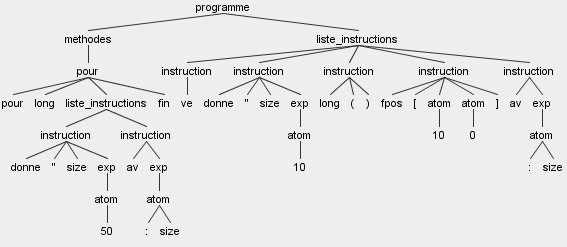
\includegraphics[width=\textwidth]{img/var_tree}
		\subcaption{Arbre}
	\end{subfigure}
	\caption{Exemple de recherche d'une variable}
\end{figure}

\section{Principe expression 'loop'}
L'expression 'loop' donne la possibilité de récupérer le nombre d'itérations qui ont été effectuées dans la boucle 'répète'. 

Initialement, il y avait une variable au niveau du LogoTreeVisitor qui stockait la valeur de l'itération de la boucle 'répète'. Il ne restait plus qu'à retourner cette valeur lorsque 'loop' était appelée. 

Cette technique fonctionnait, mais présentait un inconvénient majeur dès que des boucles 'répète' étaient imbriquées. Puisqu'il n'existait qu'une seule variable pour les différentes boucles, une fois remonté dans la hiérarchie de l'arborescence des boucles, il n'était pas possible de retrouver la valeur de l'itération de la boucle parente. 

Afin de résoudre ce problème, une pile a été créée. Dès qu'une boucle commence la valeur de l'itération est ajoutée au dessus de la pile, les instructions sont exécutées, et avant la prochaine itération la valeur au dessus de la pile est retirée. 

Ainsi, lorsque 'loop' observe la valeur au sommet de la pile, il s'agira de la valeur de l'itération de la boucle courante.

Les boucles peuvent être imbriquées sans perdre le compte dans le nombre des itérations. 
\begin{lstlisting}[language=Python]
ve
fpos [-200 0]
repete 7
[
	fcc loop
	repete 100
	[
		av 1*loop
		td 300
	]
	fpos [(-200+100*(loop+1)) 0]	
]
\end{lstlisting}

\begin{figure}[!h]
	\centering
	\begin{subfigure}[t]{.5\textwidth}
		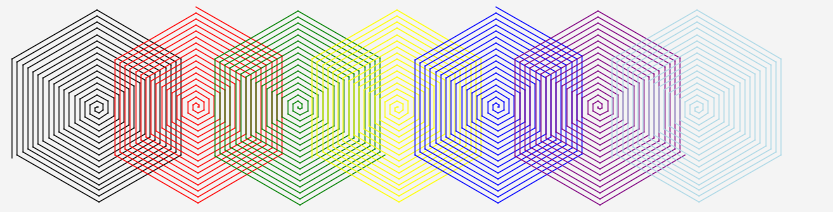
\includegraphics[width=\textwidth]{img/loop_figure}
		\subcaption{Dessin}
	\end{subfigure}
	~
	\begin{subfigure}[t]{0.7\textwidth}
		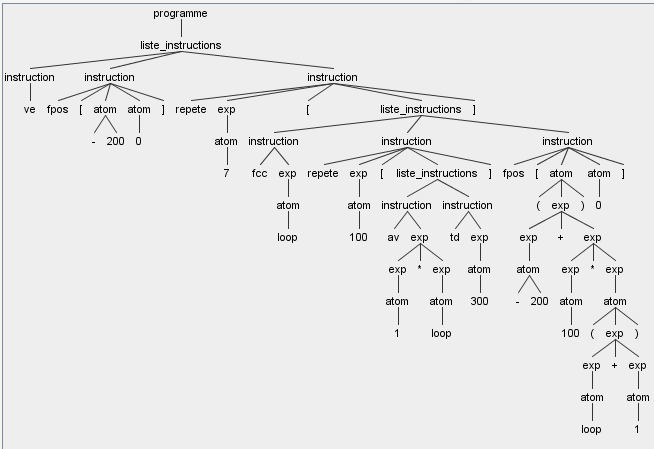
\includegraphics[width=\textwidth]{img/loop_tree}
		\subcaption{Arbre}
	\end{subfigure}
	\caption{Exemple repete imbriquées avec utilisation de loop}
\end{figure}

\section{Principe retour des fonctions}
Les fonctions sont déclarées de la même manière que les procédures, à la différence près qu'elles contiennent une instruction rends en fin de déclaration, avant 'fin'. Cependant, leur appel est différent. Comme nous l'avons vu précédemment, alors que l'appel des procédures se fait au niveau des instructions, celui des fonctions se fait au niveau des expressions, car son retour doit être évalué comme tel.

'rends' est traitée comme une directive particulière et non comme une instruction, afin de pouvoir différencier les fonctions des procédures à leur déclaration, et éviter que cette directive soit incluse dans la liste des instructions de la fonction.

Lors de l'appel de la fonction, la valeur évaluée par rends à partir de son expression associée est retournée.

Une fonction peut n'avoir que 'rends' et pas d'instruction,contrairement à une procédure, dans notre implémentation.

\begin{lstlisting}[language=Python]
pour draw :cote :couleur
	fcc :couleur
	repete 6 
	[ av :cote  	td 360/6 ]
fin
pour doubleDraw :n :iteration
	donne t  :n*2
	si :iteration > 0 
		[draw (
			doubleDraw (	:t  (:iteration - 1))
			 :iteration )
		]
	rends :t
fin
ve
doubleDraw (1 6)
\end{lstlisting}
\begin{figure}[!h]
	\centering
	\begin{subfigure}[t]{.2\textwidth}
		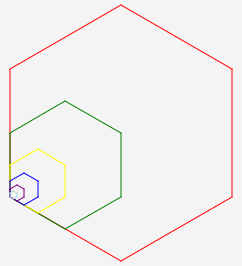
\includegraphics[width=\textwidth]{img/function_figure}
		\subcaption{Dessin}
	\end{subfigure}
	~
	\begin{subfigure}[t]{\textwidth}
		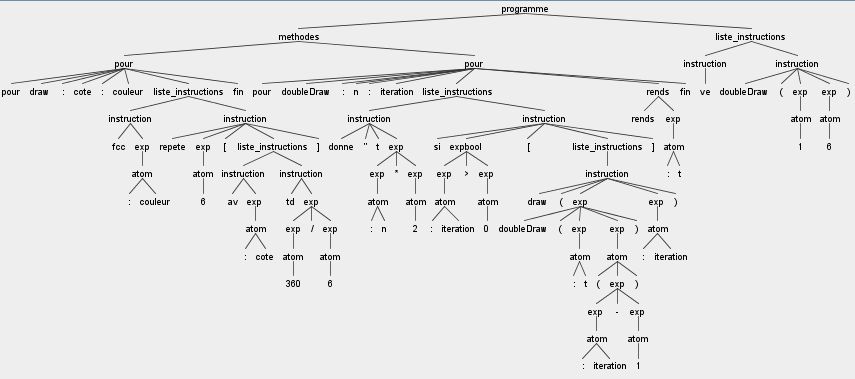
\includegraphics[width=\textwidth]{img/function_tree}
		\subcaption{Arbre}
	\end{subfigure}
	\caption{Exemple fonctions récursives}
\end{figure}

% Commentaires
\end{document}
